\documentclass[11pt]{article}
\usepackage[margin=0.9in]{geometry}
\usepackage{amsmath,amssymb,mathtools}
\usepackage{dsfont}
\usepackage{xcolor}
\usepackage{tikz}
\usepackage{microtype}
\usepackage[colorlinks=true,linkcolor=blue!55!black,urlcolor=blue!55!black]{hyperref}

\newcommand{\Tr}{\operatorname{Tr}}
\newcommand{\Np}{N'}
\definecolor{cP}{HTML}{2A78D6}
\definecolor{cPp}{HTML}{EB6834}
\definecolor{cX}{HTML}{8E2C8A}
\tikzset{
  Parc/.style={line width=3.4pt, cP},
  Pparc/.style={line width=3.4pt, cPp},
  chP/.style={line width=1.0pt, cP!85!black},
  chPp/.style={line width=1.0pt, cPp!90!black},
  chX/.style={line width=1.15pt, cX, dash pattern=on 3.2pt off 1.8pt},
  Umark/.style={draw=black, fill=white, rectangle, inner sep=1.8pt, line width=0.8pt},
  pt/.style={circle, fill=black, inner sep=1.3pt},
}
\newcommand{\chord}[4][]{\draw[#1] ({#2}:{#4}) .. controls ({#2}:{0.32*#4}) and ({#3}:{0.32*#4}) .. ({#3}:{#4});}
\newcommand{\Umk}[2]{\node[Umark] at ({#1}:{#2}) {};}

\title{\bf The $m=2$ decoder moment in terms of $Q$ and $Q^\dagger$}
\author{\small Companion to \texttt{progress\_2026-09-29.pdf}, Fig.~1 and \S3.2}
\date{30 September 2026}
\setlength{\parskip}{2pt}

\begin{document}
\maketitle

\section{Ingredients}
\paragraph{Supercharge.} One-flavor $\mathcal N{=}2$ SYK on $\Np$ complex fermions, with $p$ odd ($p=3$):
\begin{equation}
Q=\sum_{|I|=p}C_I\,\psi_I,\qquad Q^\dagger=\sum_{|I|=p}\bar C_I\,\psi_I^\dagger,\qquad
\psi_I=\psi_{i_1}\cdots\psi_{i_p}\ (i_1<\dots<i_p),
\end{equation}
with complex Gaussian couplings. Their only nonzero second moment is
\begin{equation}
\mathbb E\big[C_I\bar C_J\big]=\delta_{IJ},\qquad \mathbb E\big[C_IC_J\big]=\mathbb E\big[\bar C_I\bar C_J\big]=0 .
\label{eq:cov}
\end{equation}
(The physical variance only rescales $\beta$ below, so we set it to 1.) A \textbf{chord} is one Wick pair
$C_I\bar C_I$. It always joins a $Q$ to a $Q^\dagger$. $Q$--$Q$ and $Q^\dagger$--$Q^\dagger$ pairs vanish by
\eqref{eq:cov}.

\paragraph{The BPS projector contains both $Q$ and $Q^\dagger$.} With $H=\{Q,Q^\dagger\}=QQ^\dagger+Q^\dagger Q\ge0$,
\begin{equation}
P=\lim_{\beta\to\infty}e^{-\beta H}\Big|_{\Lambda^F}
=\lim_{\beta\to\infty}\sum_{a\ge0}\frac{(-\beta)^a}{a!}\,H^a .
\end{equation}
Since $Q^2=0$ (odd $p$), $H^a=(QQ^\dagger)^a+(Q^\dagger Q)^a$ for $a\ge1$. \emph{Every word in $P$ alternates and contains
equally many $Q$'s and $Q^\dagger$'s.} This is why chords can live inside $P$.

\paragraph{Parity probe.} $U=(-1)^{n_i}$ gives $U\psi_iU=-\psi_i$ and $U\psi_jU=\psi_j$ for $j\neq i$, so
\begin{equation}
U\psi_IU=s_I\,\psi_I,\qquad s_I\equiv(-1)^{[i\in I]},\qquad
UQU=\sum_Is_IC_I\psi_I,\qquad UQ^\dagger U=\sum_Is_I\bar C_I\psi_I^\dagger .
\label{eq:sign}
\end{equation}
Hence $P'\equiv UPU$ is the same function of the \emph{sign-flipped} couplings $C_I\to s_IC_I$.

\section{Where the $U$'s go}
\paragraph{Three $P$'s become two arcs.} $(PUP)^2=PUPUP$ has three $P$'s, but under the trace cyclicity and $P^2=P$ give
\begin{equation}
\Tr\big[(PUP)^2\big]=\Tr[P\,U\,P\,U\,P]=\Tr[P\,P\,U\,P\,U]=\Tr[P\,U\,P\,U].
\end{equation}
On the chord circle, the first and last $P$ are adjacent segments of a single arc.

\paragraph{Moving $U$ does not make it disappear for free.} $UP=(UPU)\,U=P'U$, so
\begin{equation}
\Tr[P\,U\,P\,U]=\Tr[P\,(UPU)]=\Tr[P\,P'].
\end{equation}
The two $U$'s annihilate, \emph{but the $P$ they passed is now $P'$}. By \eqref{eq:sign}, every supercharge in that arc
carries a sign $s_I$.

\section{Explicit expansion}
Expand both projectors:
\begin{equation}
\Tr\big[e^{-\beta_1H}\,U\,e^{-\beta_2H}\,U\big]=\sum_{a,b\ge0}\frac{(-\beta_1)^a(-\beta_2)^b}{a!\,b!}\,\Tr\big[H^a\,H'^{\,b}\big],
\qquad H'=UHU .
\end{equation}

\subsection*{Lowest nontrivial order: $a=b=1$}
Write
\begin{equation}
H=\sum_{I,J}C_I\bar C_J\,A_{IJ},\qquad A_{IJ}\equiv\psi_I\psi_J^\dagger+\psi_J^\dagger\psi_I,
\qquad
H'=UHU=\sum_{K,L}s_Ks_L\,C_K\bar C_L\,A_{KL}.
\end{equation}
Then
\begin{equation}
\Tr[H\,U\,H\,U]=\Tr[H\,H']=\sum_{I,J,K,L}s_Ks_L\;C_I\bar C_J\,C_K\bar C_L\;\Tr\big[A_{IJ}A_{KL}\big].
\end{equation}
By \eqref{eq:cov} the Gaussian average has exactly two Wick pairings:
\begin{equation}
\mathbb E\big[C_I\bar C_J\,C_K\bar C_L\big]=\underbrace{\delta_{IJ}\,\delta_{KL}}_{\text{(i)}}+\underbrace{\delta_{IL}\,\delta_{JK}}_{\text{(ii)}} .
\end{equation}

\paragraph{(i) No joining chord.} $Q$ pairs with $Q^\dagger$ inside $H$, and $Q'$ with $Q'^\dagger$ inside $H'$:
\begin{equation}
\text{(i)}=\sum_{I,K}\underbrace{s_K^2}_{=1}\,\Tr\big[A_{II}A_{KK}\big]=\sum_{I,K}\Tr\big[A_{II}A_{KK}\big].
\end{equation}
The chord inside the $P'$-arc carries $s_K$ at \emph{both} ends, so the signs cancel. Weight 1.

\paragraph{(ii) Two joining chords.} Chord $I$ joins the $Q$ in $H$ to the $Q'^\dagger$ in $H'$. Chord $K$ joins the
$Q^\dagger$ in $H$ to the $Q'$ in $H'$:
\begin{equation}
\text{(ii)}=\sum_{I,K}s_I\,s_K\;\Tr\big[A_{IK}A_{KI}\big].
\end{equation}
Each joining chord carries \emph{one} sign, from its end in the $P'$-arc.

\begin{figure}[!ht]
\centering
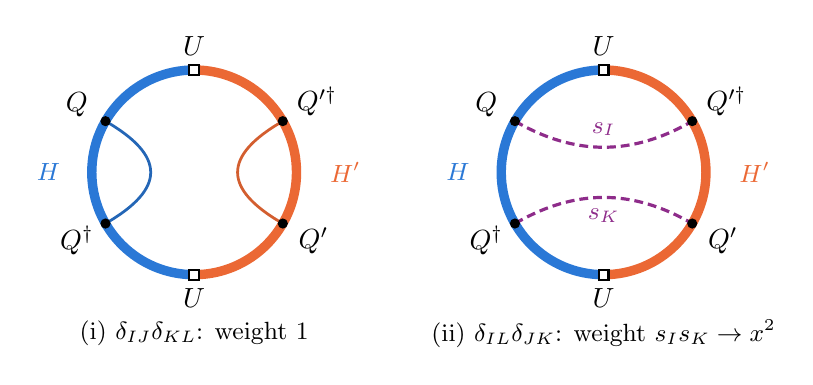
\begin{tikzpicture}
\def\R{1.3}
\foreach \xs/\lab in {0/{(i) $\delta_{IJ}\delta_{KL}$: weight $1$}, 5.2/{(ii) $\delta_{IL}\delta_{JK}$: weight $s_Is_K\to x^2$}}{
\begin{scope}[xshift=\xs cm]
  \draw[Parc] (90:\R) arc[start angle=90, end angle=270, radius=\R];
  \draw[Pparc] (-90:\R) arc[start angle=-90, end angle=90, radius=\R];
  \Umk{90}{\R}\Umk{270}{\R}
  \node at (90:\R+0.3) {$U$}; \node at (270:\R+0.3) {$U$};
  \node at (150:\R+0.42) {$Q$}; \node at (210:\R+0.42) {$Q^\dagger$};
  \node at (330:\R+0.45) {$Q'$}; \node at (30:\R+0.5) {$Q'^\dagger$};
  \node[cP] at (180:\R+0.55) {\small $H$}; \node[cPp] at (0:\R+0.62) {\small $H'$};
  \node[font=\small] at (0,-2.05) {\lab};
\end{scope}}
\chord[chP]{150}{210}{\R}
\chord[chPp]{330}{390}{\R}
\begin{scope}[xshift=5.2cm]
  \chord[chX]{150}{30}{\R}
  \chord[chX]{210}{330}{\R}
  \node[cX] at (0,0.55) {\small $s_I$}; \node[cX] at (0,-0.55) {\small $s_K$};
\end{scope}
\foreach \xs in {0,5.2}{\begin{scope}[xshift=\xs cm]
  \foreach \a in {150,210,330,30} {\node[pt] at (\a:\R) {};}
\end{scope}}
\end{tikzpicture}
\caption{The two Wick pairings of the term $\Tr[Q\,Q^\dagger\,U\,Q'\,Q'^\dagger\,U]$ in $\Tr[HUHU]$ (read
counterclockwise from the top). Blue: $P$-arc. Orange: $P'$-arc. Squares: $U$. A chord whose endpoints lie on opposite
sides of a $U$ carries one sign $s_I$. The pairing $Q$--$Q'$, $Q^\dagger$--$Q'^\dagger$ would give a single crossing
diagram, but it vanishes by \eqref{eq:cov}.}
\end{figure}



\paragraph{No single joining chord.} $H$ holds one $Q$ and one $Q^\dagger$. If its $Q$ pairs across, its $Q^\dagger$
has no partner left except across.

\section{All orders}
In $\Tr[H^aH'^{\,b}]$, the summand for fixed indices is the same fermion trace as in $\Tr[H^{a+b}]$. The only
difference is a factor $s_I$ on each primed supercharge. After Wick contraction:
\begin{itemize}\itemsep1pt
\item a chord inside the $P$-arc carries no sign;
\item a chord inside the $P'$-arc carries $s_I^2=1$;
\item a chord joining the arcs carries exactly one $s_I$.
\end{itemize}
Hence
\begin{equation}
\Tr[H^a H'^{\,b}]=\sum_{\text{pairings }\pi}\ \sum_{\text{indices}}\Big(\prod_{c\,\in\,\text{joining}(\pi)}s_{I_c}\Big)\times
\big[\text{summand of }\Tr(H^{a+b})\text{ for }\pi\big].
\end{equation}
All crossing weights ($q$-factors) sit in the fermion trace and are unchanged by $U$. The probe contributes only
the signs.

\paragraph{Joining chords come in pairs.} The $P$-arc word has $a$ $Q$'s and $a$ $Q^\dagger$'s. Each internal chord
uses one of each, since $Q$--$Q$ pairs vanish. The ends left over to join across are therefore balanced: $n$ $Q$-ends
and $n$ $Q^\dagger$-ends, i.e.\ $2n$ joining chords.

\paragraph{Averaging the signs.} For a uniformly random $p$-subset, $\Pr[i\in I]=p/\Np$, so
\begin{equation}
\overline{s_I}=1-\frac{2p}{\Np}\equiv x\qquad(\text{exact, one chord}).
\end{equation}
If the $2n$ signs are replaced independently by their mean, a diagram with $2n$ joining chords is weighted by $x^{2n}$.
Taking $\beta_{1,2}\to\infty$ and resumming gives
\begin{equation}
T_2=\tau(PP')=\sum_{n\ge0}P_n\,x^{2n},
\end{equation}
with $P_n$ the probability that the zero-temperature wormhole has $n$ chords (BLY eqs.~4.5--4.8 with $\lambda=2p^2/\Np$,
$\Delta=1/p$; in that limit $x\simeq e^{-2p/\Np}=q^{1/p}$).

\paragraph{Caveat (finite $N$).} Replacing each $s_{I_c}$ by $x$ \emph{independently} is the double-scaled
approximation. At finite $N$, the fermion trace (e.g.\ $\Tr[A_{IK}A_{KI}]$) depends on how $I$ and $K$ overlap,
including whether $i$ lies in both. So the weighted average of $s_Is_K$ is not exactly $x^2$. The exact finite-$N$
statement for $T_2$ is the size sum rule of \S4 of the progress report, which needs no chord factorization.

\end{document}
